% \documentclass[hcross_theory.tex]{subfiles}
\documentclass{standalone}

\usepackage{tikz}
\usetikzlibrary{backgrounds}
\usetikzlibrary{math}
\usepackage{multirow}

\usetikzlibrary{
    positioning, 
    calc, 
    % external, 
    patterns, 
    arrows.meta, 
    shapes.arrows, 
    shapes.misc}
\usepackage{tikz-3dplot}


\begin{document}

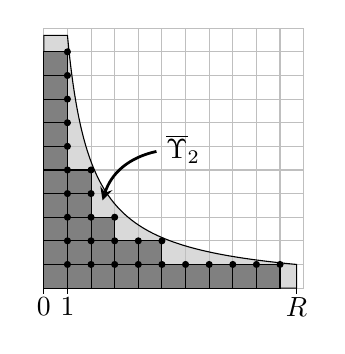
\begin{tikzpicture}[scale=0.3]
\newcommand{\hcrossouterradiustikz}{10.7}
\newcommand{\hcrossinnerradiustikz}{9.7}
\newcommand{\hcrossnxnytikz}{11}

\fill[fill=gray!30] plot[smooth, samples=100, domain=1:\hcrossouterradiustikz] (\x, \hcrossouterradiustikz / \x) -- (\hcrossouterradiustikz, 0) -- (0, 0) -- (0, \hcrossouterradiustikz) -- cycle;

\draw[lightgray] (0,0) grid (\hcrossnxnytikz,\hcrossnxnytikz);

\draw plot[smooth, samples=100, domain=1:\hcrossouterradiustikz] (\x, \hcrossouterradiustikz / \x) -- (\hcrossouterradiustikz, 0) -- (0, 0) -- (0, \hcrossouterradiustikz) -- cycle;

\foreach \x in {0,1,...,\hcrossnxnytikz}
{
\foreach \y in {0,1,...,\hcrossnxnytikz}
{
\pgfmathsetmacro{\Jn}{ifthenelse(\x*\y<=\hcrossouterradiustikz,ifthenelse(\x<=\hcrossouterradiustikz,ifthenelse(\y<=\hcrossouterradiustikz,ifthenelse(\x>0,ifthenelse(\y>0,1,0),0),0),0),0)}
\ifthenelse{\Jn=1}
{
    \path [fill=gray,draw=black] (\x-1.0,\y-1.0) rectangle (\x-0.0,\y-0.0);
}
{}
}
}

\foreach \x in {0,1,...,\hcrossnxnytikz}
{
\foreach \y in {0,1,...,\hcrossnxnytikz}
{
\pgfmathsetmacro{\Jn}{ifthenelse(\x*\y<=\hcrossouterradiustikz,ifthenelse(\x<=\hcrossouterradiustikz,ifthenelse(\y<=\hcrossouterradiustikz,ifthenelse(\x>0,ifthenelse(\y>0,1,0),0),0),0),0)}
\ifthenelse{\Jn=1}
{
    \node[draw,circle,inner sep=0.75pt,fill,color=black] at (\x,\y) {};
}
{}
}
}

\draw (0,0)--(0,-.25);

\draw (1,0)--(1,-.25);

\draw (\hcrossouterradiustikz,0)--(\hcrossouterradiustikz,-.25);

\node[below] at (0,0) {$0$};
\node[below] at (1,0) {$1$};
\node[below] at (\hcrossouterradiustikz,0) {$R$};

\node (A) at (2.3,3.3) {};
\node (B) at (5.9,5.9) {$\overline{\Upsilon}_2$};

\draw[thick,->,>=stealth, line width=0.35mm] (B) edge[bend right] (A);

\end{tikzpicture}

\end{document}